\chapter{Redes sociales}

\section{Modelo del votante Barabasi-Albert y S-M}

\subsubsection{\large Simular el modelo del votante en una red pequeño mundo y en una red de Barabási-Albert y estudiar su comportamiento emergente} 
El modelo de votante es un modelo de no equilibrio que tiene solucion analitica en cualquier dimension. Tendriamos N agentes sociales, nodos de una red. Cada agente puede estar en dos estados ($\pm1$). Cada paso temporal es elegido un agente y uno de sus vecinos y adquieren el mismo estado.

Red de pequeño mundo:

En la figura se puede ver el aspecto de nuestra red \ref{1} (se ha creado segun los estándares, pero el output de python es bastante reducido). El aspecto final \ref{2}. Y la fraccion a lo largo del tiempo, propia de estos sistemas complejos: \ref{3}.
\begin{figure}
	\centering
	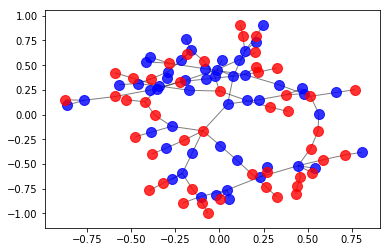
\includegraphics[width=9cm]{dist_inic_small}
	\caption{Estado inicial para red pequeño mundo}
	\label{1}
\end{figure}

\begin{figure}
	\centering
	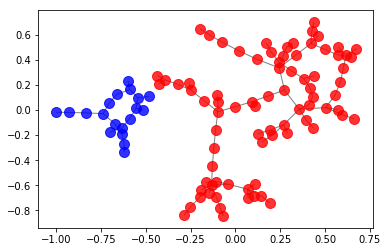
\includegraphics[width=9cm]{final_small}
	\caption{Estado final (Se representa distinto para observar mejor la clusterizacion)}
	\label{2}
\end{figure}

\begin{figure}
	\centering
	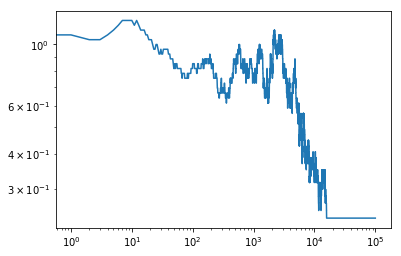
\includegraphics[width=9cm]{frac_small}
	\caption{Fracción de pares con distinta opinión en función del tiempo en un modelo del votante}
	\label{3}
\end{figure}

Red de Barabási-Albert:

En la figura se puede ver el aspecto de nuestra red \ref{4} (se ha creado segun los estándares, pero el output de python es bastante reducido). El aspecto final\ref{5}. Y la fraccion a lo largo del tiempo, propia de estos sistemas complejos: \ref{6}.
En este caso vemos algunas incoherencias, pero son comprensibles debido al bajo numero de nodos de nuestra red (por limitaciones de mi ordenador).
\begin{figure}
	\centering
	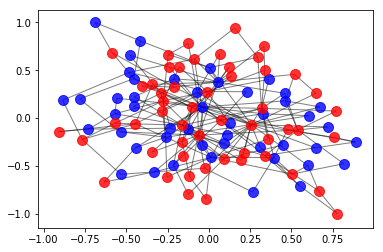
\includegraphics[width=9cm]{barra_inic}
	\caption{Estado inicial para red pequeño mundo}
	\label{4}
\end{figure}

\begin{figure}
	\centering
	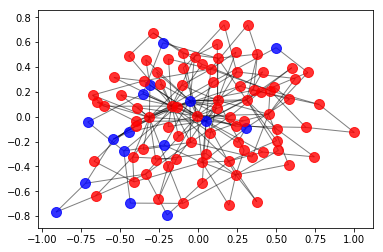
\includegraphics[width=9cm]{barra_fin}
	\caption{Estado final}
	\label{5}
\end{figure}

\begin{figure}
	\centering
	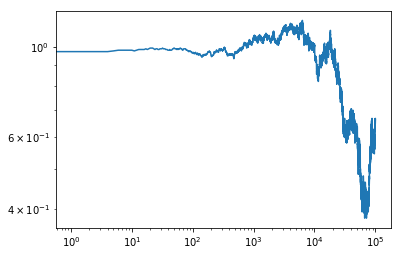
\includegraphics[width=9cm]{barra_frac}
	\caption{Fracción de pares con distinta opinión en función del tiempo en un modelo del votante}
	\label{6}
\end{figure}

\section{Competicion de lenguas}
\subsubsection{\large Estudiar las soluciones del sistema anterior y su estabilidad e interpretar cada uno de los estados estacionarios posibles.} 

Estamos ante el estudio del sistema de competición de lenguas, que viene dictaminado por la ecuación:
$$dm_A/dt=s(m_A)^a(1-m_A)-(1-s)(1-m_A)^am_A$$
Esta ecuacion tiene 3 puntos de equilibrio para $a\neq1$:
Si $a>1$ tenemos $m_A=0$ y $m_A=1$ como puntos de equilibro estables, aquellos en los que alguna otra lengua elimina a la competencia. Tenemos otro punto critico entre 0 y 1 que representa un estado inestable de equilibrio entre las lenguas.

Para $a<1$ el problema es el mismo pero la cualidad de estabilidad se invierte en los puntos criticos encontrados.
(Se ha consultado para este apartado el articulo \textit{Microscopic Abrams-Strogatz model of language competition})
